\documentclass[a4paper]{report}
\usepackage{pdfpages}
\usepackage[utf8]{inputenc}
\usepackage[slovak]{babel}
\usepackage{graphicx}
\usepackage{xcolor}
\usepackage{environ}
\usepackage{ifmtarg}
\usepackage{amssymb,amsmath}
\usepackage{listings}
\usepackage{lmodern}
\usepackage{rotating}
\usepackage{setspace}
\usepackage{etoolbox}
\usepackage{caption}
\usepackage{subcaption}
\usepackage[framemethod=default]{mdframed}
\usepackage{fullpage}
\usepackage{verbatim}
\usepackage[unicode]{hyperref}

\definecolor{lightyellow}{rgb}{1.0,1.0,0.7}

\newcommand{\todoin}[1]{\fcolorbox{red}{red}{\color{yellow}\textbf{TODO: }}\fcolorbox{red}{lightyellow}{#1}}
\newcommand{\todo}[1]{\todoin{#1}\linebreak}
\newcommand{\bigtodo}[1]{\begin{mdframed}[frametitle={\color{yellow}\textbf{TODO:}},
 frametitlebackgroundcolor=red,
 backgroundcolor=lightyellow,
 skipbelow=2mm,
 linecolor=red,
 innertopmargin=.8\baselineskip] #1 \end{mdframed}}

\makeatletter
\newcommand{\labelname}[1]{
  \def\@currentlabelname{#1}}%
\makeatother

\newcommand{\zadanietpl}[3][]{
\medbreak
\refstepcounter{section}
\labelname{#2}%
\addcontentsline{toc}{section}{\protect\numberline{\thesection} #2}
\ifstrequal{#1}{}{}{\label{#1}}
\nopagebreak
\begin{mdframed}
\vspace{0.7em}
{\large \textbf \thesection} \quad {\large \textbf {#2}}
\nopagebreak
#3
\nopagebreak
\vspace{0.7em}
\end{mdframed}
\vspace{1 em}
}

\NewEnviron{zadanie}[2][]{%
\zadanietpl[#1]{#2}{\vspace{1.25 em} \BODY}
}

\newcommand{\kzadanie}[2][]{
\zadanietpl[#1]{#2}{}
}

\newcommand{\zadanieref}[1]{\hyperref[#1]{\nameref*{#1} (\ref*{#1})}}

\begin{document}
\begingroup % predok
\pagenumbering{roman}
\tableofcontents
\endgroup % predok

\newpage
\pagenumbering{arabic}
\setcounter{page}{1}

\chapter{Databázy}

\begin{zadanie}{Účel databáz, charakteristika DB aplikácií, trojstupňová ANSI/SPARC architektúra, koncepčné dátové modely, navrhovanie databáz}

\begin{itemize}
 \item Entitno-relačný a relačný dátový model.
 \item Entitno-relačné diagramy, UML diagramy.
 \item Motivácia normalizácie.
\end{itemize}
\end{zadanie}

\begin{zadanie}{Teória navrhovania databáz}

\begin{itemize}
 \item Funkčné závislosti, Armstrongove axiómy.
 \item Uzáver množiny atribútov, uzáver množiny funkčných závislostí.
 \item Pokrytie a minimálne pokrytie množiny funkčných závislostí.
 \item Nadkľúče a kľúče.
 \item Relačné schémy, dekompozícia relačných schém, bezstratovosť dekompozície.
 \item Normálne formy: 3NF, BCNF.
 \item Naivná dekompozícia do 3NF a BCNF.
 \item Dekompozícia do 3NF zachovávajúca funkčné závislosti.
\end{itemize}
\end{zadanie}

\begin{zadanie}{Dotazovacie jazyky}
\begin{itemize}
 \item Relácie a predikáty, dotazy, relačný kalkul, Datalog, SQL, relačná algebra.
 \item Vyjadrovacia sila a vzájomné simulácie dotazovacích jazykov.
\end{itemize}
\end{zadanie}

\begin{zadanie}{Agregácia a rekurzia v dotazovacích jazykoch}
\begin{itemize}
 \item Grupovanie a agregácia v relačnej algebre, SQL, relačnom kalkule a Datalogu.
 \item Rekurzia v relačnej algebre, SQL, relačnom kalkule a Datalogu.
\end{itemize}
\end{zadanie}

\begin{zadanie}{Výpočet rekurzívnych programov a programov s negáciou}
\begin{itemize}
 \item Naivná evaluácia, seminaivná evaluácia.
 \item Unifikácia, SLD rezolúcia, rule-goal-tree, rule-goal-graph, väzby medzi premennými (binding patterns).
 \item Magická transformácia.
 \item Modely, stratifikovaná negácia, stable a well-founded sémantika.
\end{itemize}
\end{zadanie}

\begin{zadanie}{Optimalizácia dotazov}
\begin{itemize}
 \item Strom relačného výrazu.
 \item Optimalizácia konjunktívnych dotazov dekompozíciou hypergrafu, Wong-Youssefiho algoritmus.
 \item Optimalizácia pomocou semijoinov, úplný reduktor, Yannakakisov algoritmus.
\end{itemize}
\end{zadanie}

\begin{zadanie}{Optimalizácia konjunktívnych dotazov}
\begin{itemize}
 \item Pohltenie (containment) a ekvivalencia konjunktívnych dotazov.
 \item Testovanie pohltenia, petrifikované dotazy.
 \item Optimalizácia za predpokladu slabej ekvivalencie.
 \item Tablá a ich použitie.
\end{itemize}
\end{zadanie}

\begin{zadanie}{Transakcie}
\begin{itemize}
 \item Definícia transakcie, elementárne transakčné operácie, požiadavky na transakčný systém.
 \item Komponenty transakčného databázového systému.
 \item Rozvrhy, triedy rozvrhov.
 \item Konflikt-sériovateľnosť, testovanie konflikt-seriovatelnosti, view-sériovateľnosť, dvojfázové zamykanie, obnova.
 \item Striktné dvojfázové zamykanie, riešenie deadlockov.
 \item Časové pečiatky, validácia.
\end{itemize}
\end{zadanie}

\begin{zadanie}{Fyzická organizácia}
\begin{itemize}
 \item Fyzická algebra, zložitosť fyzických operátorov.
 \item Sekvenčné indexy, B stromy a B+ stromy.
 \item Hashovanie.
 \item Štruktúra hashovaného súboru: adresár, základné bloky, bloky preplnenia.
 \item Rozšíriteľné hashovanie.
 \item Lineárne hashovanie.
 \item Implementácia a zložitosť vybraných fyzických operátorov (merge-sort, nested-loop-join, ...).
\end{itemize}
\end{zadanie}

\begin{zadanie}{Distribuované databázy}
\begin{itemize}
 \item Atomický commit, výber koordinátora (bully algoritmus), replikácia dát.
 \item Distribuované zámky, distribuované deadlocky.
 \item Synchronizácia času, Christianov algoritmus, Berkeley algoritmus.
\end{itemize}
\end{zadanie}

\paragraph*{Úvod}

Transakcia:
\begin{itemize}
 \item program pristupuúci k databáze
 \item môže ich bežať viacero v tom istom čase
 \item postupnosť operácií R, W, INSERT, DEL, START, COMMIT, ABORT
\end{itemize}

\begin{description}
\item[Atomicity]
celá transakcia zbehne, alebo sa nevykoná vôbec

\item[Consistency]
vykonanie T z konz. stavu do konz. stavu

\item[Isolation]
výsledok rovnaký ako keď transakcie sú serializované

\item[Durability]
ak T úspešne skončí, tak zmeny ostanú navždy zachované
\end{description}

\begin{minipage}[t]{0.5\textwidth}
\centerline{Centralizovaná DB}
\begin{itemize}
 \item[+] jednoduchá, spoľahlivá
 \item[+] kompatibilná s $\exists$ byrokraciou
 \item[-] výpadok centrály
 \item[-] rýchlosť obsluhovania požiadaviek
\end{itemize}
\end{minipage}
\begin{minipage}[t]{0.5\textwidth}
\centerline{Distribuovaná DB}
\begin{itemize}
 \item[+] odolnosť voči výpadkom
 \item[+] rýchlosť
 \item[-] komplikovaná archit., bezpečnosť, integrita
 \item[-] cena, chýbajúce štandardy a skúsenosti
 \item[-] databázový dizajn komplikovaný
\end{itemize}
\end{minipage}

\hrule

\begin{description}
\item[horizontálna fragmentácia]
rovnaké dáta na rôznych miestach: pobočky banky

\item[vertikálna fragmentácia]
rôzne dáta na rôznych miestach: štátne inštitúcie
\end{description}

Požiadavky:

\begin{itemize}
 \item ACID, transparentnosť (jedno na kt. pobočke)
 \item odolnosť voči výpadkom uzlov a liniek
\end{itemize}

\hrule
\noindent
Zvyšok viď \zadanieref{sec:distribuovany-commit}, \zadanieref{sec:distribuovana-replikacia-db} a \zadanieref{sec:synchronizacia-casu}

\chapter{Distribuované systémy}

\begin{zadanie}{Vrstvové modely}
\begin{itemize}
 \item vrstvy, služby, rozhrania (interfaces), referenčný model OSI
 \item TCP/IP, úlohy jednotlivých vrstiev
\end{itemize}
\end{zadanie}

\begin{zadanie}{Sieťová vrstva v TCP/IP}
\begin{itemize}
 \item adresácia v TCP/IP, protokoly IP, ARP, ICMP
 \item routovanie (smerovanie) v TCP/IP, NAT
\end{itemize}
\end{zadanie}

\begin{zadanie}{Transportná vrstva v TCP/IP}
\begin{itemize}
 \item úlohy a služby transportnej vrstvy
 \item protokoly UDP a TCP
\end{itemize}
\end{zadanie}

\begin{zadanie}{Fyzická a linková vrstva}
\begin{itemize}
 \item Ethernet, CSMA/CD
 \item rozširovanie Ethernetu na fyzickej a linkovej vrstve – huby, switche, WiFi, CSMA/CA
\end{itemize}
\end{zadanie}

\begin{zadanie}{Domain Name System (DNS)}
\begin{itemize}
 \item doménové meno, úloha DNS, architektúra DNS
 \item typy záznamov, reverzné vyhľadávanie
\end{itemize}
\end{zadanie}

\begin{zadanie}{Bezpečnostné mechanizmy na linkovej vrstve}
\begin{itemize}
 \item VLAN
 \item riadenie prístupu k portu na báze linkovej adresy
 \item IEEE 802.1X, bezpečnosť WiFi
\end{itemize}
\end{zadanie}

\begin{zadanie}{Bezpečnostné mechanizmy na sieťovej a transportnej vrstve}
\begin{itemize}
 \item firewall
 \item IPSec
 \item SSL/TLS
\end{itemize}
\end{zadanie}

\begin{zadanie}{Bezpečnosť elektronickej pošty a webu}
\begin{itemize}
 \item problémy a riešenia, end-to-end security
 \item PGP, S/MIME
 \item komunikácia so serverom (IMAPS, POP3S, SMTPS)
 \item HTTPS, certifikáty
\end{itemize}
\end{zadanie}

\begin{zadanie}{Model komunikácie so zdieľanou pamäťou}
\begin{itemize}
 \item POSIX thready, vytváranie, ukončovanie a finálna synchronizácia threadov.
 \item Zdieľané premenné, mutex, conditional variable.
 \item Scheduling.
\end{itemize}
\end{zadanie}

\begin{zadanie}{Thready v Jave}
\begin{itemize}
 \item Vytváranie threadov, ukončovanie threadov.
 \item Synchronizácia prístupu k metódam a premenným.
 \item Synchronizácia na úrovni tried a na úrovni objektov.
 \item Scheduling.
\end{itemize}
\end{zadanie}

\begin{zadanie}{Kanálový model komunikácie}
\begin{itemize}
 \item Synchrónna a asynchrónna kanálová komunikácia.
 \item sémantika posielania a prijímania správ.
\end{itemize}
\end{zadanie}

\begin{zadanie}{Point-to-point model komunikácie}
\begin{itemize}
 \item Synchrónna a asynchrónna point-to-point komunikácia.
 \item Sémantika posielania a prijímania správ.
\end{itemize}
\end{zadanie}

\begin{zadanie}[sec:distribuovany-commit]{Problém Commitu v distribuovaných databázach}
\begin{itemize}
 \item Atomický commit, výber koordinátora (bully algoritmus).
\end{itemize}
\end{zadanie}

\paragraph{Atomický commit protocol}

\begin{itemize}
 \item $\forall$ čo urobia rozhodn. $\rightarrow$ rovnaké (ABORT/COMMIT)
 \item keď sa proces rozhodne, už svoje rozhodnutie nezmení
 \item COMMIT len ak $\forall$ hlasujú YES
 \item ak $\forall$ YES a $\nexists$ výpadky $\Rightarrow$ musí byť COMMIT
 \item ak po výpadku dlho ďaľšie nie sú \ldots musí byť rozhodnuté
\end{itemize}

\noindent
asynchr. model komunikácie, jeden uzol koordinátor (ost. participanti)

\subparagraph*{2-fázový}
\begin{enumerate}
 \item hlasovanie (koord. vyzve k hlasovaniu, part. pošlú hlasy)
 \item koord. čaká na hlasy, globálne rozhodnutie (koord. pošle rozhodnutie)
 \item[final] koord. čaká na ACK
\end{enumerate}

\begin{itemize}
 \item ak spadne PART
 \begin{itemize}
  \item ak to koord zistí \ldots ABORT
 \end{itemize}
 \item ak spadne KOORD
 \begin{itemize}
  \item ak niekto má COMMIT/ABORT tak sa ostatní informujú
  \item ak $\forall$ YES - problém BLOCK kým sa koord. neobnoví
 \end{itemize}
\end{itemize}

\subparagraph*{3-fázový}
\begin{itemize}
 \item pridávanie PRECOMMIT fázy
 \item ak spadne KOORD
 \begin{itemize}
  \item ak má niekto PRECOMMIT $\rightarrow$ COMMIT
  \item ak $\nexists \rightarrow$ ABORT
  \item nekonzistencia ak graf rozdelený na 2 komp.
 \end{itemize}
\end{itemize}

\subparagraph*{Majoritný 3-fázový}
\begin{itemize}
 \item posielanie PREABORT
 \item rozhodnutie ak väčšina uzlov PREABORT / PRECOMMIT
\end{itemize}

\paragraph{Bully algoritmus na výber koordinátora}

\begin{itemize}
 \item iniciátor posiela $\uparrow$ id správu Election
 \item tí, čo nie sú spadnutí pošlú OK
 \item tí, čo poslali OK robia to, čo iniciátor
 \item ak niekto nepošle OK spať: oznám $\forall$ menším, že som koord.
\end{itemize}

\begin{zadanie}[sec:distribuovana-replikacia-db]{Replikácia dát v distribuovaných databázach}
\begin{itemize}
 \item Replikácia dát.
 \item Distribuované zámky, distribuované deadlocky.
\end{itemize}
\end{zadanie}

\paragraph{Replikácia dát}
\begin{itemize}
 \item rovnaké dáta na rôznych miestach (zabezp. izoláciu a sériov.)
 \item čítanie dát možné z ľubov. uzla, write treba vo všetkých
\end{itemize}

\paragraph{Distribuované zamykanie}
\subparagraph*{centralizovaná schéma}
\begin{itemize}
 \item len jeden uzol je lock manager (+jednoduché, -malá odolnosť, -bottleneck)
\end{itemize}

\subparagraph*{primary copy schéma}
\begin{itemize}
 \item každý uzol je lock manager zodpovedný za podmnožinu dát
 \item read-lock možno žiadať od hociktorého LM
 \item write-lock možno žiadať len od primárneho LM (len 1 kóp. je primárna), ten konzultuje s ostatnými, čo majú danú kópiu
\end{itemize}

\noindent
(+ menší bottleneck, -možnosť distr. deadlocku)

\subparagraph*{2-fáz. Read-One-Write-All (ROWA) protokol}
\begin{itemize}
 \item RL hocikto, kto má dáta
 \item WL treba žiadať všetkých, čo majú dané dáta
\end{itemize}

\subparagraph*{Majoritný 2-fáz. protokol}
\begin{itemize}
 \item na RL aj WL treba žiadať väčšinu lock managerov
 \item deadlock môže nastať aj pri zamykaní 1 záz. (3. trans. vlastna každá 1/3 zámkov. workaround: poradie zamykania lockov)
\end{itemize}

\subparagraph*{Quorum protokol}
\begin{itemize}
 \item Každý uzol váha $w_i$, $w_i > 0$
 \item $Q_r,Q_w > 0:\:Q_r + Q_w > \Sigma w_i \wedge 2 Q_w > \Sigma w_i$
 \item Každý read (resp. write) musí získať zámok na toľkých kópiách, aby suma uzlov, ktoré tie kópie spravujú bola aspoň $Q_r$ (resp. $Q_w$)
\end{itemize}

\paragraph{Správa deadlockov}
\begin{itemize}
 \item uzly majú lokálny wait-for graf (WFG)
 \item koordinátor robí globálny WFG, ak nájde cyklus $\rightarrow$ ABORT
 \item problém: detekcia $\nexists$ cyklov (glob. WFG je len aproximácia, kvôli oneskoreniam/poradiu správ o lok. WFG, preto koord. niekedy abortne aj transakcie, ktoré nemusí)
\end{itemize}

\begin{zadanie}[sec:synchronizacia-casu]{Synchronizácia času v distribuovaných systémoch}
\begin{itemize}
 \item Synchronizácia fyzických hodín, Christianov algoritmus, Berkeley algoritmus.
 \item Lamportov čas.
\end{itemize}
\end{zadanie}

\paragraph{Synchronizácia fyzických hodín}
\begin{itemize}
 \item $\forall$ uzol má lokálne hodiny
 \item $\forall$ hodiny len dopredu
 \item rôzne hodiny môžu mať rôzne fyzické časy
 \item rôzne hodiny môžu tikať rôzne rýchlo
\end{itemize}

\paragraph{Christianov algoritmus}
\begin{itemize}
 \item klienti si synchr. čas podľa jedného servera
 \item ak I nepoznáme: kom. čas = $(T_1 - T_0) / 2$
 \item ak I poznáme: kom. čas = $(T_1 - T_0 - I) / 2$
 \item nastav hodiny na $C_UTC$ + kom. čas (ak je to menej, spomaľ hodiny, aby za zaručilo,
 že idú vždy dopredu)
\end{itemize}

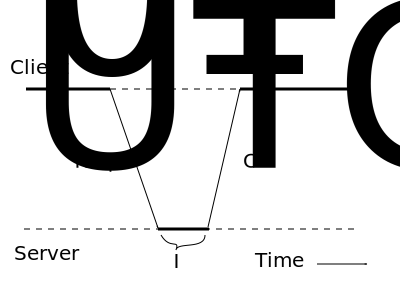
\includegraphics[width=0.5\textwidth]{obrazky/christianov-protokol}

\paragraph{Berkeley protokol}
\begin{itemize}
 \item server synchronizuje čas všetkých na priemer
\end{itemize}
\begin{enumerate}
 \item server pošle svoj čas
 \item $\forall$ odpovedia rozdielom
 \item server zpriemeruje a pošle každému o koľko si má posunúť hodiny
\end{enumerate}

\paragraph{Logické hodiny}
\begin{itemize}
 \item čas. pečiatky pre udalosti
 \item Ak $A_i$ po $A_j$ potom $C(A_i) > C(A_j)$
 \item Ak $A_i$ prijatie správy v procese P a $A_j$ odoslanie správy z P, potom $C(Ai) < C(Aj)$
 \item $\forall i,j: C(A_i) \neq C(A_j)$
\end{itemize}

\paragraph{Lamportov čas}
\begin{itemize}
 \item buď si každý posunie hodiny dopredu, ak obdrží správu s vyššou pečiatkou ako je jeho aktúálny čas
 \item alebo (alternatívna implementácia), časová pečiatka je n-tica obsahujúca najväčšie známe časy v jednotlivých uzloch, sled udalostí = lexikografické usporiadanie, synchr. fyz. hodín nie je nutná (iba to, že idú dopredu)
\end{itemize}

\chapter{OO analýza}

\kzadanie{Use-case modelovanie}
\kzadanie{Modelovanie tried}
\kzadanie{Modelovanie kompozitných štruktúr}
\kzadanie{Modelovanie interakcií}
\kzadanie{Modelovanie stavových automatov}
\kzadanie{Modelovanie aktivít}
\kzadanie{Modelovanie komponentov}
\kzadanie{Modelovanie nasadenia systému}
\kzadanie{Pomocné modelovacie konštrukty}
\kzadanie{UML profily}

\chapter{Teória paralelných výpočtov}

\begin{zadanie}{Paralelné gramatiky}
\begin{itemize}
 \item paralelné prepisovanie
 \begin{itemize}
  \item Lindenmayerove systémy
  \item Indické a Ruské paralelné gramatiky
  \item generatívne systémy
 \end{itemize}
 \item kooperujúce distribuované gramatiky
 \item paralelné gramatické systémy
\end{itemize}
\end{zadanie}

\begin{zadanie}{Paralelné stroje}
\begin{itemize}
 \item alternujúce Turingove stroje
 \item alternujúce konečné automaty
 \item boolovské obvody
 \item PRAM
 \item počítače druhej triedy
\end{itemize}
\end{zadanie}

\begin{zadanie}{Ťažké problémy}
\begin{itemize}
 \item Trieda NC
 \item redukovateľnosť
 \item P-úplné problémy
\end{itemize}
\end{zadanie}

\chapter{Výpočtová zložitosť}

\begin{zadanie}{Turingove stroje, základné zložitostné triedy a vzťahy medzi nimi}
\begin{itemize}
 \item Savitchova veta
 \item simulácie a hierarchie
\end{itemize}
\end{zadanie}

\kzadanie{Gap Theorem a Veta o zrýchľovaní}
\begin{zadanie}{NP-úplnosť, Cook-Levinova veta}
a niektoré ďalšie (aj pre prax dôležité) NP-úplné problémy
\end{zadanie}
\kzadanie{Vzťah NP-úplných a NP-optimalizačných problémov}
\kzadanie{Aproximačné algoritmy pre NP-optimalizačné problémy; neaproximovateľnosť}

\begin{zadanie}{Pravdepodobnostné algoritmy}
\begin{itemize}
 \item Veta o vylepšovaní
 \item BPP vs. PSPACE
\end{itemize}
\end{zadanie}

\chapter{Vypočítateľnosť}

\begin{zadanie}{Churchova-Turingova téza}
\begin{itemize}
 \item Zdôvodnenie ekvivalencie Turingovych strojov počítajúcich funkciu a Minského registrových strojov.
\end{itemize}
\end{zadanie}

\begin{zadanie}{Primitívna rekurzia}
\begin{itemize}
 \item Definícia tejto triedy funkcií a základné vlastnosti.
 \item Súvis s programami bez while-cyklov.
\end{itemize}
\end{zadanie}

\begin{zadanie}{Rekurzívne a čiastočne rekurzívne funkcie}
\begin{itemize}
 \item Definícia a ekvivalencia s automatovými modelmi vypočítateľnosti.
 \item Rekurzívne množiny a predikáty.
\end{itemize}
\end{zadanie}

\begin{zadanie}{Aritmetizácia syntaxe}
\begin{itemize}
 \item Kódovanie objektov do čísel.
 item Univerzálne funkcie a ich zložitosť vzhľadom na príslušnú triedu funkcií.
\end{itemize}
\end{zadanie}

\begin{zadanie}{Vyčísliteľné reálne čísla}
\begin{itemize}
 \item Definícia a základné vlastnosti.
\end{itemize}
\end{zadanie}

\begin{zadanie}{Nerozhodnuteľné problémy}
\begin{itemize}
 \item Funkcia Busy Beaver.
 \item Problém zastavenia a jeho úplnosť pri many-to-one redukcii.
\end{itemize}
\end{zadanie}

\chapter{Vyhľadávanie v texte}

\begin{zadanie}{Vyhľadávanie vzorky v texte}
\begin{itemize}
 \item pomocou konečných automatov
 \item Knuth-Morris-Prattov algoritmus
\end{itemize}
\end{zadanie}

\kzadanie{Sufixové stromy a príklady ich použitia}
\kzadanie{Sufixové polia}
\kzadanie{Výpočet editačnej vzdialenosti medzi reťazcami}
\kzadanie{Výpočet najdlhšej spoločnej podpostupnosti dvoch reťazcov}
\kzadanie{Vyhľadávanie približných výskytov vzorky v texte}

\chapter{Kompilátory}

\begin{zadanie}{Štruktúra kompilátorov}
\begin{itemize}
 \item Základné pojmy. Vzťah k teórii jazykov. Syntaktická analýza. Sémantika. Jedno a viac prechodové kompilátory.
 \item Jednoduchý jednoprechodový kompilátor. Rekurzívny zostup. Syntaktické diagramy.
\end{itemize}
\end{zadanie}

\begin{zadanie}{Lexikálna analýza}
\begin{itemize}
 \item Dôvody oddelenia lexikálnej a syntaktickej analýzy. Lexikálna štruktúra jazykov. Regulárne jazyky. Konečné automaty.
 \item Syntéza: Regulárny jazyk - nedeterministický konečný automat - deterministický konečný automat.
\end{itemize}
\end{zadanie}

\begin{zadanie}{Syntaktická analýza}
\begin{itemize}
 \item Bezkontextové gramatiky. Návrh gramatiky jazyka. Syntaktické stromy.
 \item Metódy zhora - dolu: rekurzívny zostup, LL(1), LL(k).
 \item Metódy zdola - hore: Operátorovo precedenčné gramatiky a jazyky, LR(k) metódy ( SLR(1), LALR(1)).
 \item Oprava chýb a zotavenie sa z chýb pri syntaktickej analýze.
\end{itemize}
\end{zadanie}

\begin{zadanie}{Syntaxou riadené preklady}
\begin{itemize}
 \item Atribútové gramatiky. Syntetizované a zdedené atribúty.
 \item Vyhodnocovanie atribútov. Porovnanie metód zhora - dole a zdola - hore.
 \item Graf závislosti atribútov.
\end{itemize}
\end{zadanie}

\begin{zadanie}{Kontrola typov}
\begin{itemize}
 \item Systém typov v programovacích jazykoch a konverzie medzi typmi.
 \item Gramatika typov a kontrola typov ako syntaxou riadený preklad.
 \item Polymorfické typy. Unifikácia.
\end{itemize}
\end{zadanie}

\begin{zadanie}{Podpora v čase behu (Run-time environments)}
\begin{itemize}
 \item Organizácia a prideľovanie pamäte.
 \item Odovzdávanie parametrov, lokálne a nelokálne premenné.
 \item Prideľovanie a organizácia dynamickej pamäte.
 \item Tabuľka symbolov - hašovanie.
\end{itemize}
\end{zadanie}

\begin{zadanie}{Generovanie medzijazyka}
\begin{itemize}
 \item Formy medzijazyka:
 \begin{itemize}
  \item Poľská bezzátvorková forma
  \item trojadresový kód
  \item trojice, štvorice
 \end{itemize}
 \item Generovanie medzijazyka syntaxou riadeným prekladom.
 \item Popis základných konštrukcii: deklarácie, výrazy, príkaz priradenia, booleovské výrazy, podmienené príkazy a cykly. Volanie procedúr a funkcií.
 \item Spätné plátanie (backpatching).
\end{itemize}
\end{zadanie}

\begin{zadanie}{Generovanie kódu}
\begin{itemize}
 \item Cieľový počítač: CISC, RISC, SIC. Ceny inštrukcií.
 \item Administrácia pamäte. Statická pamäť, zásobník, dynamická pamäť - heap.
 \item Prideľovanie registrov. Prideľovanie registrov farbením grafu.
 \item Generovanie kódu z dagu.
 \item Generovanie kódu pokrývaním ozdobeného stromu.
\end{itemize}
\end{zadanie}

\begin{zadanie}{Optimalizácia kódu}
\begin{itemize}
 \item Kukátková (peephole) optimalizácia.
 \item Optimalizácia základných blokov, optimalizačné transformácie.
\end{itemize}
\end{zadanie}

\chapter{Kolmogorovská zložitosť}

\begin{zadanie}{Definícia, význam a základné vlastnosti Kolmogorovskej zložitosti}
\begin{itemize}
 \item Varianty Kolmogorovskej zložitosti a vzťahy medzi nimi
\end{itemize}
\end{zadanie}

\begin{zadanie}{Nestlačiteľné reťazce}
\begin{itemize}
 \item definícia, význam.
 \item Vysvetlenie metódy nestlačiteľnosti a ukážka jej využitia na konkrétnych príkladoch.
\end{itemize}
\end{zadanie}

\end{document}